\chapter{Analisi}

\section{Analisi nomi-verbi}
A questo punto partendo dalla specifica si vogliono identificare gli oggetti e le operazioni nel sistema, individuando alcune parole chiave: 

\begin{itemize}
\item In \textbf{grassetto} vengono evidenziati i nomi, che potranno essere classi.
\item In \textit{corsivo} vengono evidenziati i verbi, che identificano operazioni o servizi, i metodi delle classi.
\item In \underline{sottolineato} gli attributi. 
\end{itemize}


Progettare un sistema di prenotazione  di \textbf{posto} a lezione, nel rispetto della (nuova) \underline{capienza} delle \textbf{aule} (caratterizzate da un \underline{codice}). La presenza degli \textbf{studenti} è organizzata in \textbf{turni} \textit{prenotabili} in base alle ultime due cifre del numero di \underline{matricola} (da 00 a 49 e da 50 a 99) a settimane alterne. La prenotazione per ciascun turno può essere \textit{fatta} (e \textit{cancellata}, per permettere a studenti in lista d’attesa di \textit{frequentare}) solo dal lunedì a venerdì della settimana precedente. Al termine della prenotazione, il sistema \textit{produce} una \textbf{ricevuta} (con\underline{aula}, \underline{matricola} ed \underline{orario}) da \textit{scaricare/salvare}. Per \textit{accedere} al sistema servono le \textbf{credenziali} di Sapienza.





\section{Schede CRC}
Le schede CRC (\textit{Class, Responsibility, Collaboration})  descrivono in modo semplice e veloce le classi di analisi estratte con l'analisi nomi-verbi.
Ciascuna scheda descrive una classe (o un oggetto) indicando \footnote{Alcune implemenmtazioni delle schede CRC presentano anche gli attributi dell’oggetto o della classe, in questo caso non sono stati inseriti ma sono visibili nella sezione ~\ref{sec: dati} inerente alla specifica dei dati.}:
\begin{enumerate}
\item Il nome della classe (\textit{class}).
\item Le sue superclassi e sottoclassi.
\item Le sue responsabilità, ovvero le azioni che permette di svolgere o che svolge (\textit{responsibility}).
\item Il nome di altre classi con cui questa classe collabora per svolgere i compiti di cui è responsabile (\textit{collaboration}).
\end{enumerate}
\medskip
  
 
\begin {tabular}{>{\bfseries}lp{10cm}}
\toprule
Nome & \textbf{Studente}\\
\midrule
Descrizione  & Classe che rappresenta un utente autenticato nel sistema.\\
%\midrule
SuperClasse & -\\
%\midrule
SottoClasse & -\\
%\midrule
Responsabilità & -\\ 
%\midrule
Collaborazioni & -\\
\bottomrule
\end {tabular}\newline

\medskip 

\begin {tabular}{>{\bfseries}lp{10cm}}
\toprule
Nome & \textbf{Utente non autenticato}\\
\midrule
Descrizione  & Classe che rappresenta un utente non ancora autenticato nel sistema.\\
%\midrule
SuperClasse & -\\
%\midrule
SottoClasse & -\\
%\midrule
Responsabilità & -\\ 
%\midrule
Collaborazioni & -\\
\bottomrule
\end {tabular}\newline

\medskip

\begin {tabular}{>{\bfseries}lp{10cm}}
\toprule
Nome & \textbf{Prenotazione}\\
\midrule
Descrizione  & Classe che modella l’oggetto prenotazione, contiene tutte le informazioni che identificano una prenotazione.\\ %agggiure richiamo alal specifica dei dati
%\midrule
SuperClasse & -\\
%\midrule
SottoClasse & -\\
%\midrule
Responsabilità & - \\
%\midrule
Collaborazioni & -\\
\bottomrule
\end {tabular}\newline


\medskip


\begin {tabular}{>{\bfseries}lp{10cm}}
\toprule
Nome & \textbf{Aula}\\
\midrule
Descrizione  & Classe che astrae il concetto di aula, contiene tutte le informazioni inerenti ad un aula.\\
%\midrule
SuperClasse & -\\
%\midrule
SottoClasse & -\\
%\midrule
Responsabilità & - \\
%\midrule
Collaborazioni & -\\
\bottomrule
\end {tabular}\newline

\medskip





\begin {tabular}{>{\bfseries}lp{10cm}}
\toprule
Nome & \textbf{RicevutaPrenotazione}\\
\midrule
Descrizione  &  Rappresenta l’oggetto ricevuta della prenotazione\\ %agggiure richiamo alal specifica dei dati
%\midrule
SuperClasse & -\\
%\midrule
SottoClasse & -\\
%\midrule
Responsabilità & - \\
%\midrule
Collaborazioni & -\\
\bottomrule
\end {tabular}\newline

\medskip

\begin {tabular}{>{\bfseries}lp{10cm}}
\toprule
Nome & \textbf{HandlerEffetuaPrenotazioni}\\
\midrule
Descrizione  & Classe che permette la gestione di una prenotazione.\\ 
%\midrule
SuperClasse & -\\
%\midrule
SottoClasse & -\\
%\midrule
Responsabilità & \begin{itemize}
\item Effettua dei controlli sulla capienza dell’aula. 
\item Effettua i controlli sulla possibilità di effettuare una prenotazione (settimana e matricola).
\item Permette di effetuare una prenotazione in base ai dati presi in input.
\item Crea una ricevuta come output della prenotazione con tutte le informazioni necessarie.
\end{itemize}\\
%\midrule
Collaborazioni & Studente, Prenotazione, Aula, RicevutaPrenotazione, HandlerInviaMail.\\
\bottomrule
\end {tabular}\newline

\medskip

\begin {tabular}{>{\bfseries}lp{10cm}}
\toprule
Nome & \textbf{HandlerCancella}\\
\midrule
Descrizione  & Classe che gestisce l’eliminazione di prenotazioni in corso.\\
%\midrule
SuperClasse & -\\
%\midrule
SottoClasse & -\\
%\midrule
Responsabilità & \begin{itemize}
\item Permette di cancellare una prenotazione.
\end{itemize}\\
%\midrule
Collaborazioni & Prenotazione.\\
\bottomrule
\end{tabular}\newline

\medskip

\begin {tabular}{>{\bfseries}lp{10cm}}
\toprule
Nome & \textbf{HandlerVisualizza}\\
\midrule
Descrizione  & Classe che gestisce la visualizzazione delle prenotazioni.\\
%\midrule
SuperClasse & -\\
%\midrule
SottoClasse & -\\
%\midrule
Responsabilità & \begin{itemize}
\item Permette di visualizzare le prenotazioni in corso con tutte le informazioni.
\item Permette di visualizzare le prenotazioni scadute.
\item Permette di visualizzare lo stato di una prenotazione.
\end{itemize}\\
%\midrule
Collaborazioni & Prenotazione, Studente.\\
\bottomrule
\end{tabular}\newline

\medskip


\begin {tabular}{>{\bfseries}lp{10cm}}
\toprule
Nome & \textbf{HandlerScarica}\\
\midrule
Descrizione  & Classe che gestsice la visualizzazione e il download delle ricevute.\\
%\midrule
SuperClasse & -\\
%\midrule
SottoClasse & -\\
%\midrule
Responsabilità & \begin{itemize}
\item Permette di visualizzare la ricevuta di una prenotazione.
\item Permette di scaricare in locale la ricevuta di una prenotazione in formato PDF.
\end{itemize}\\
%\midrule
Collaborazioni & Prenotazione, RicevutaPrenotazione, HandlerEffetuaPrenotazioni, HandlerInviaMail.\\
\bottomrule
\end{tabular}\newline

\medskip

\begin {tabular}{>{\bfseries}lp{10cm}}
\toprule
Nome & \textbf{HandlerGestisciCoda}\\
\midrule
Descrizione  & Classe che aggiunge rimuove e gestisce gli utenti in coda.\\
%\midrule
SuperClasse & -\\
%\midrule
SottoClasse & -\\
%\midrule
Responsabilità & \begin{itemize}
\item Inserisce  un utente in coda se non è possibile effettuare una prenotazione.
\item Rimuove quando necessario il primo utente dalla coda, aggiornando lo stato della prenotazione.
\end{itemize}\\ 
%\midrule
Collaborazioni & Prenotazione, Aula, Studente, HandlerInviaMail.\\
\bottomrule
\end {tabular}\newline

\medskip

\begin {tabular}{>{\bfseries}lp{10cm}}
\toprule
Nome & \textbf{HandlerInviaMail}\\
\midrule
Descrizione  & Classe che gestisce l’invio delle mail agli studenti.\\
%\midrule
SuperClasse & -\\
%\midrule
SottoClasse & -\\
%\midrule
Responsabilità & \begin{itemize}
\item Invia per mail la ricevuta della prenotazione.
\item Invia per mail eventuali aggiornamenti sullo stato della prenotazione.
\end{itemize}\\ 
%\midrule
Collaborazioni & Prenotazione, Studente, RicevutaPrenotazione, HandlerGestisciCoda, HandlerEffetuaPrenotazioni.\\
\bottomrule
\end {tabular}\newline

\medskip

\begin {tabular}{>{\bfseries}lp{10cm}}
\toprule
Nome & \textbf{HandlerLogin}\\
\midrule
Descrizione  & Classe che gestisce il login dell’utente.\\
%\midrule
SuperClasse & -\\
%\midrule
SottoClasse & -\\
%\midrule
Responsabilità & \begin{itemize}
\item Permette di effettuare il login.
\item Segnala con un errore eventuali problemi.
\end{itemize}\\
%\midrule
Collaborazioni & Studente.\\
\bottomrule
\end {tabular}\newline

\medskip

\begin {tabular}{>{\bfseries}lp{10cm}}
\toprule
Nome & \textbf{HandlerLogout}\\
\midrule
Descrizione  & Classe che gestisce il logout dell’utente.\\
%\midrule
SuperClasse & -\\
%\midrule
SottoClasse & -\\
%\midrule
Responsabilità & \begin{itemize}
\item Permette di effettuare il logout.
\item Segnala con un errore eventuali problemi.
\end{itemize}\\
%\midrule
Collaborazioni & Studente.\\
\bottomrule
\end {tabular}\newline

\medskip



\begin {tabular}{>{\bfseries}lp{10cm}}
\toprule
Nome & \textbf{UILogin}\\
\midrule
Descrzione & Classe che rappresenta l’interfaccia che permette il login all’interno del sistema.\\
%\midrule
SuperClasse & -\\
%\midrule
SottoClasse & -\\
%\midrule
Responsabilità & -\\
%\midrule
Collaborazioni & HandlerLogin.\\
\bottomrule
\end {tabular}\newline

\medskip


\begin {tabular}{>{\bfseries}lp{10cm}}
\toprule
Nome & \textbf{UILogout}\\
\midrule
Descrzione & Classe che rappresenta l’interfaccia che permette il logout dal sistema.\\
%\midrule
SuperClasse & -\\
%\midrule
SottoClasse & -\\
%\midrule
Responsabilità & -\\
%\midrule
Collaborazioni & HandlerLogout.\\
\bottomrule
\end {tabular}\newline

\medskip



\begin {tabular}{>{\bfseries}lp{10cm}}
\toprule
Nome & \textbf{UIPrenotazione}\\
\midrule
Descrzione & Classe che rappresenta l’insieme degli elementi
dell’interfaccia che permettono di effettuare una prenotazione e getsire le prenotazioni da parte di uno studente.\\
%\midrule
SuperClasse & -\\
%\midrule
SottoClasse & -\\
%\midrule
Responsabilità & -\\
%\midrule
Collaborazioni & HandlerEffetuaPrenotazioni, HandlerCancella, HandlerVisualizza, HandlerScarica, HandlerGestisciCoda, HandlerInviaMail.\\
\bottomrule
\end {tabular}\newline









\section{Stereotipi}
\begin{itemize}
\item \textbf{Entity:} classe che mantiene informazioni di lunga durata, tipicamente persistenti
\item \textbf{Boundary:} classe che modella l’interazione tra sistema e attori, spesso è un’astrazione di un elemento software di interfaccia
\item \textbf{Control:} classe che si occupa del controllo e coordinamento di altri oggetti, tipicamente è associabile a un caso d’uso.
\end{itemize}
La figura~\ref{figura: EBC} mostra il diagramma.
	

	
\begin{figure}[H]
\begin{center}
  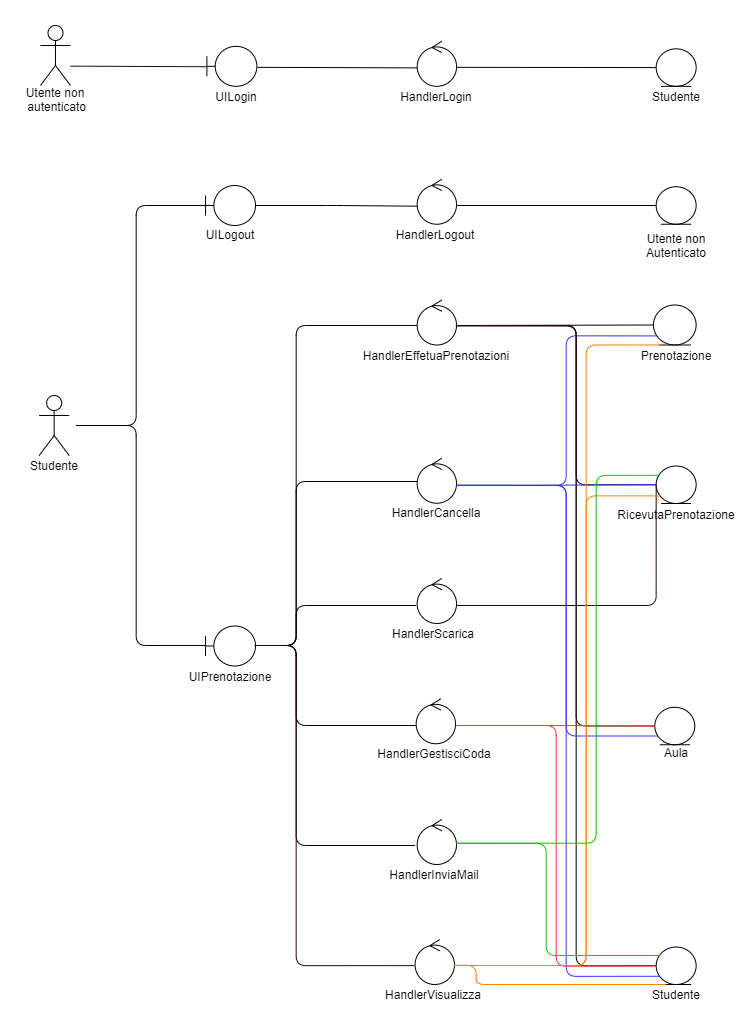
\includegraphics[width=0.8 \textwidth]{Figure/EBC.png}
    \caption{Diagrammi EBC.}\label{figura: EBC}
\end{center}
\end{figure}
	
	  

\section{Organizzazione in package}
A questo punto gli elementi individuati nelle sezioni precedenti vengono raggruppati ad alto livello in package comunicanti, la suddivisione è visibile nella figura ~\ref{figura: package} 


\begin{figure}[H]
\begin{center}
  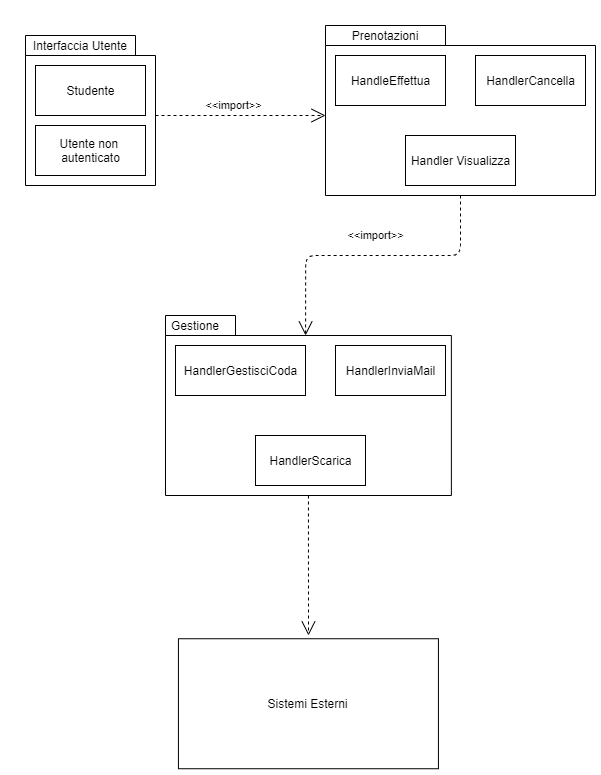
\includegraphics[width=0.8 \textwidth]{Figure/package.png}
    \caption{Organizzazione in package.}\label{figura: package}
\end{center}
\end{figure}

